\documentclass{lecturenotes}

\title[Kort presentation av pgk \& dod, 2016-08-25]{\textbf{EDAA45} Programmering, grundkurs (pgk) \\ + \\ \textbf{EDA070} Datorer och datoranvändning (dod)}
\author{\href{http://cs.lth.se/bjorn-regnell}{Björn Regnell}, \href{http://cs.lth.se/roger_henriksson}{Roger Henriksson}}
\institute{\href{http://cs.lth.se}{Datavetenskap}, LTH}
\date{2016-08-25}
 
\begin{document}

\newcommand{\DagOchPlats}{måndag kl 13:15 i E:A}
 
\frame{\titlepage}

%\SlideImg{Att lägga grunden \href{http://www.vhuset.lth.se/v-husets-bibliotek/om-v-biblioteket/byggandet-av-lth/}{...}}{img/lthgrund.jpg}
%Bilden av grundläggningen av Mattehuset, LTH från juni 1963 

\frame{\frametitle{En kurskombo som startar på \DagOchPlats}
Lägger grunden för alla kommande kurser i datavetenskap: \vspace{1em}
\begin{itemize}
\item \Alert{Programmering, grundkurs} (pgk), 7.5 hp, 16 veckor
\begin{itemize}
\item[] En grundlig genomgång av programmering \Emph{från början} \\ med stora möjligheter till \Emph{fördjupning} som du själv väljer
\end{itemize}
\vspace{1em}
\item \Alert{Datorer och datoranvändning} (dod), 3 hp, 3 veckor
\begin{itemize}
\item[] Inblick i hur datorer fungerar och verktygen vi använder
\end{itemize}
\end{itemize}
}

\frame{\frametitle{Vad ska du lära dig?}
%Att skapa koden som styr världen...
%\includegraphics[width=1.2\textwidth, height=1.5cm]{img/code-wide}
\begin{multicols}{2}
\begin{itemize}\Size{9pt}
\item \textbf{Programmering, grundkurs}
\begin{itemize}\Size{8pt}
\item Tänka i abstraktioner
\item Använda datastrukturer
\item Implementera algoritmer
\item Brepp som lägger grunden för resten av din utbildning
\item Språk: \Emph{Scala} och Java
\end{itemize}
\columnbreak
\item \textbf{Datorer \& datoranvändning}
\begin{itemize}\Size{8pt}
\item Lågnivåprogrammering
\item Internet
\item Terminalkommando i Linux
\item Skriva \& typsätta i \LaTeX
\item Beräkningar i Matlab
\end{itemize}
\end{itemize}
\end{multicols}
\vspace{1em}
\flushright\scriptsize Denna presentation i \LaTeX ~på GitHub:\\\url{https://github.com/lunduniversity/introprog/}
}

%%%
\frame{\frametitle{Hur ska du lära dig?}
\begin{itemize}
\item Genom praktiskt eget arbete: Lära genom att göra!
\begin{itemize}
\item Övningar
\item Laborationer
\item Projekt
\end{itemize}
\item Genom studier av begrepp: Skapa förståelse
\item Genom samarbete med dina kurskamrater
\end{itemize}
}

\SlideImg{Det brukar vara stor spridning i programmeringsförkunskaper bland D-are \\(enkätsvar 2015)}{../img/survey-2015}

%%%
\frame[plain]{\frametitle{Förkunskapsenkät}

Ditt svar på denna \Emph{förkunskapsenkät} används i planeringen:
\url{http://cs.lth.se/pgk/survey}\\
\Alert{Fyll i enkäten redan idag!}\\
\vspace{1em}
Enkäten innehåller dessa frågor och några till:
\begin{itemize}
\item Har du programmerat tidigare? \\
         Ja \hspace{2.5cm} Nej 
\item Hur många program har du skrivit? \\ 
         $<5$ \hspace{2.2cm} $5-20$ \hspace{2.5cm}  $>20$
\item Hur stort var det största program du har skrivit?\\ 
         $<50$ rader \hspace{1cm} $50 - 500$  rader \hspace{1cm}  $>500$ rader
\end{itemize}
\vspace{1em}
}

%%%
\frame{\frametitle{Kurslitteratur} 
\footnotesize
\begin{columns}
\begin{column}{0.65\textwidth}
{\Size{16pt}pgk:}
\begin{itemize}
\item \Emph{Kompedium}: \\ \Alert{''Introduktion till programmering \\med Scala och Java''}\\ Säljs till självkostnadspris på institutionen efter beställning på första föreläsningen. \\ Ladda ner: \url{http://cs.lth.se/pgk}
\end{itemize}
\vspace{1em}
{\Size{16pt}dod:}
\begin{itemize}
\item Kursmaterial delas ut på första föreläsningen.
\end{itemize}
\end{column}
\begin{column}{0.35\textwidth}
\centering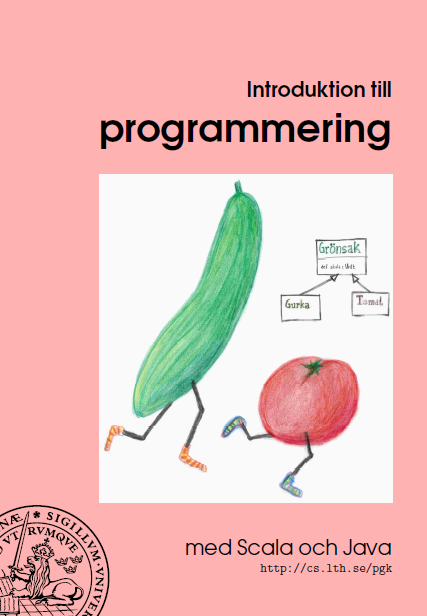
\includegraphics[width=0.99\textwidth]{../img/compendium-front-page}
\end{column}
\end{columns}


}

\SlideImg{Välkommen på \DagOchPlats}{../img/ehuset}


\end{document}

